%\section{Experiments}
%\label{sec:experiments}
\section{Short Tutorial on Q-learning}

\subsection{Reinforcement learning problem}

An RL problem is formalized as an Markov Decision Process (MDP). A MDP is
defined by a four tuple $(\State, \Action, \Trans, \Rew)$, where $\State$ is the
state space, $\Action$ is the action space, $\Trans : \State \times \Action
\rightarrow \State$ is the system dynamics and $\Rew : \State \times \Action
\rightarrow \R $ is the reward function
In a typical RL problem the transition function $\Trans$ is not given but is
known to be static.
The objective of a typical RL problem is to maximize the expected cumulative
reward over time, called the returns  $R_t = \sum_{t^{'}=t}^{T} \rew_{t^{'}}$.

\subsection{Notation}

\begin{tabular}{ll}   
  \toprule
  Symbol & Meaning\\
  \midrule
  $\state \in \State$ & State $\state$ in state space $\State$ \\
  $\act \in \Action$ & Action $\act$ in Action space $\Action$ \\
  $\rew \in \R$ & Observed reward \\
  $\goal \in \Goal$ & Goal $\goal$ in goal space $\Goal$ \\
  $f_\goal(\state_t): \State \rightarrow \Goal$ & Function to compute achieved goal \\
  $\Rew(\state, \act) : \State \times \Action \rightarrow \R $ & Reward function \\
  $\Rew(\state, \goal, \act) : \State \times \Goal \times \Action \rightarrow \R $ & Goal-conditioned Reward function \\
  $\TransFull$ & Transition function \\
  $\discount$ & Discount factor \\
  MDP=$(\State, \Action, \Trans, \Rew, \discount)$& Markov Decision Process \\
  $\policy(\state): \State \rightarrow \Action $ & Policy function \\
  $\policy(\state, \goal): \State \times \Goal \rightarrow \Action $ & Goal conditioned Policy function \\
  $\Q_\policy(\state, \act; \param_\Q) = \E_\policy[ \sum_{k=t}^\infty \discount^{k-t} \Rew(\state_k, \act_k) | \state_t = \state, \act_t = \act ] $ & $Q$-function \\
  $\Q^*(\state, \act; \param_\Q) = \arg \max_\policy \Q_\policy(\state, \act; \param_\Q)$ & Optimal $Q$-function \\
  $\fwargs{\state}{\act}{\goal^*}{\policy}{} = \E_\policy[ \sum_{k=t}^\infty \discount^{k-t}\Rew(\state_k, \goal^*, \act_k) | \state_t = \state, \act_t = \act]$ & Goal conditioned Q-function \\
  \bottomrule
\end{tabular}

\subsection{Background: Q-Learning}

Q-learning works by maintaining an action-value function $\Q : \State \times
\Action \rightarrow \R$ which is defined as the expected cumulative reward
  $\Q_\policy(\state, \act; \param_\Q) = \E_\policy[ \sum_{k=t}^\infty
  \discount^{k-t} \Rew(\state_k, \act_k) | \state_t = \state, \act_t = \act ]$
  starting from a given state-action pair.
The Q-learning algorithm works by updating the $\Q$-function using the Bellman
equation for every transition from $\state$ to $\state'$ on action $\act$
yielding reward $\rew$, 
%
\begin{align}
\Q^*(\state_t, \act_t; \param_\Q) &\leftarrow \Rew(\state_t, \act_t) + \discount \max_{\act \in \Action} \Q^*(\state_{t+1}, \act; \param_\Q)
                                    \label{eq:bellman}
\end{align}

A greedy policy can be computed from $\Q^*$-function easily $\policy^*(\state_t) = \arg \max_{\act \in \Action} \Q^*(\state_t, \act)$.

\subsection{Background: Deep Q-Learning}

\citet{MnKaSiNATURE2015} introduced neural network version of Q-learning, Deep
Q-Networks (DQN) with
two main ideas
%
\begin{enumerate}
\item For learning to be stable using bellman equation two set of parameters
  $\param_{\Q}$ should be maintained target parameters
  $\param_{\Q_t}$ and main parameters $\param_{\Q_m}$. The
  target parameters are a moving average of the main parameters that change
  slowly than main parameters. The loss function is only optimized for main parameters:
\begin{align}
  \Loss_t(\param_{\Q_m}) = \left(
  \Q^*(\state_t, \act_t; \param_{\Q_m}) -
  \Rew(\state_t, \act_t) + \discount \max_{\act \in \Action} \Q^*(\state_{t+1}, \act; \param_{\Q_t}) \right)^2
                                    \label{eq:bellman-dqn}
\end{align}

\item Since the transitions from an episode or a trajectory are not
  independently distributed, we should maintain a replay buffer in which the
  transitions are stored and then resampled at random to update the Q-function
  using Bellman equation~\eqref{eq:bellman}
\end{enumerate}%
% 


\subsection{Background: Deep deterministic policy-gradients}

Deep deterministic policy-gradients (DDPG)~\citep{lillicrap2015continuous}
extends DQN~\citep{MnKaSiNATURE2015} to continuous action domains by introducing
a parameterized policy function $\policy(\state; \param_\policy)$. The loss
function now becomes
\begin{align}
  \Loss(\param_{\Q_m}, \param_{\policy_m}) = \E_{a_t\sim\policy(\state_t; \param_{\policy_m})}\left[
  \Q^*(\state_t, \act_t; \param_{\Q_m}) -
  \Rew(\state_t, \act_t) + \discount \Q^*(\state_{t+1}, \policy(\state; \param_{\policy_t}); \param_{\Q_t}) \right]^2 \label{eq:bellman-ddpg}
\end{align}

Note that the $\max_{\act \in \Action}$ has been replaced with choosing an action
using the target policy $\policy(\state; \param_{\policy_t})$ and the actions
$\act_t$ are being sampled from the main policy. Hence the $\param_{\policy_m}$
is updated using policy gradients:
%
\begin{align}
\nabla_{\param_{\policy_m}} \Loss \propto \frac{1}{N} \sum_t \nabla_\act \Q^*(\state_t, \act; \param_{\Q_m})\nabla_{\param_{\policy_m}} \policy(\state_t; \param_{\policy_m})
\end{align}%
% 

\subsection{Goal conditioned tasks}
These tasks need the specification of goal state which can change for each trial~\citep{plappert201802multigoalrl}. The
examples include navigation to a goal location, moving a robotic arm so that the
tip of the arm is at a particular 3D location (Fetch-Reach task).

At the start of the task, a state space $\State$ (example: joint angles of the
arm), an action space $\Action$ (example: keypresses for discrete actions, joint
torques for continuous actions), and a
Goal space $\Goal$ (example: 3D coordinates of the destination location).
It is known that the transition function $\TransFull$
and the reward function $\Rew: \State \times \Action \times \Goal \rightarrow
\R$ are static.
At the start of each episode, a goal state $\goal^* \in \Goal$ is given. At each
step $t$ the agent can chose an action to take $\act_t$ and can observe
$(\state_t, \goal_t, \rew_t)$ where $\goal_t$ is the achieved goal which can be
deterministically computed from state $\goal_t = f_\goal(\state_t)$.
The reward function is formulated such that reward for reaching at the goal
$\|\goal_t - \goal^*\|_2 < \epsilon$ once
is higher than reward for visiting any other state $\infty$-times
$\Rew(\state_g, \goal^*, \act) \ge
\frac{1}{1-\discount}\max_{\state, \act'}\Rew(\state, \goal^*,
\act') \forall \act$, where $\state_g$ is such that $\|f_\goal(\state_g) -
\goal^*\| < \epsilon$.

We use Fetch push, reach and pick and place
tasks~\citep{plappert201802multigoalrl} in our experiments:
%
\begin{description}
  \item[Fetch-Reach] The tip of a robotic arm reaching a desired location.
  \item[Fetch-Push] A robotic arm pushing a block to a desired location.
  \item[Fetch-Slide] A robotic arm sliding a puck to a desired location.
\end{description}%
% 
\subsection{Baseline: Hindsight experience replay}
Hindsight Experience Replay~\cite{andrychowicz2016learning} targets
goal-conditioned tasks.
In goal-conditioned tasks, the rewards can be very sparse. Unless the agent hits
the goal, no value-able reward is learned and rest of the space is almost even
with respect to the rewards. To address this challenge, HER first assumes that
for every $\state_t$ the achieved goal $\goal_t = f_\goal(\state_t)$ is known.
Then HER simulates as if the achieved goal $\goal_t$ was the intended goal all
along by re-sampling the goal conditioned reward function.
More concretely, two time steps $t_1$ and $t_2 > t_1$ from the same episode in the replay memory are
sampled. The achieved goal at $t_2$ , $\goal_{t_2}$ is assumed to be the desired
goal at $t_1$ and the new simulated transition becomes $(\state_{t_1},
\act_{t_1}, \state_{t_1 + 1}, \Rew(\state_{t_1}, \goal_{t_2}, \act_{t_1}))$,
where $\Rew(\state_{t_1}, \goal_{t_2}, \act_{t_1})$ is the recomputed reward
instead of the observed reward $\Rew(\state_{t_1}, \goal^*_{e}, \act_{t_1})$ that
depends on the desired goal $\goal^*_{e}$ for that episode $e$.

HER can be applied to either DDPG or DQN, the experiments in
\citet{andrychowicz2016learning} show them to be applied on DDPG.

\subsection{Goal conditioned tasks: Alternative formulation}
Unlike \citet{andrychowicz2016learning}, we do not believe that reward
information is meaningless without achieving the desired goal state.

We make three assumptions:
\begin{enumerate}
\item We assume that there is no special reward
  on reaching a particular state even the goal state. The reward formulation is
  static even with change in goal states.
  In a graph interpretation, this equivalent to assuming that there are no
  vertex rewards but only edge rewards.
  $\Rew(\state, \goal, \act) = \Rew(\state, \act)$.
\item Like the Floyd-Warshall algorithm we assume no positive reward cycles
  exist i.e. $  \sum_{k=t}^{T-1} \Rew(\state_k, \act_k) \le 0 \text{ if }\state_T = \state_t$.
\end{enumerate}

The benefit of these assumptions is that we do not need to resample the reward
function with simulated goals as HER~\cite{andrychowicz2016learning} need to do.
Resampling the reward function can be expensive.

\subsection{Proposed algorithm: Floyd-Warshall RL}

We present a model-free reinforcement learning method that transfers
learned behavior when goal locations are dynamic. We call this algorithm
Floyd-Warshall Reinforcement Learning, because of its similarity to
Floyd-Warshall algorithm~\cite{floydwarshall1962}:
a shortest-path planning algorithm on graphs. Similar
to universal value function~\cite{schaul2015universal}, we define the Floyd-Warshall
(FW) function as the expected cumulative reward on going from a start
state to an end state:
%
\begin{align}
\fwargs{\state_t = \state}{\act_t = \act}{\goal}{\policy}{} =
\E_{\act_k \sim \policy(\state_t),T}\left[ \sum_{k=t}^{T-1} \Rew(\state_k, \act_k) \middle\vert \state_t = \state, \act_t = \act, \|f_\goal(\state_T) - \goal\|_2 < \epsilon \right] ,
\end{align}%
%

Note that objective is different from reinforcement learning formulated in HER,
as it is conditioned on the goal now. In \citet{andrychowicz2016learning}, the
reward formulation has to reflect that the desired goal to reach. In our formulation
we make it a precondition to the objective function, hence we do not need to
make the reward function dependent upon goal.
We want to find the policy that maximizes the expected reward from any
state $\state_t$ to a desired goal $\goal$:
%
\begin{align}
  \policy^* &=
\arg \max_{\policy} \E_{\state_t, \act_k \sim \policy(\state_t), T}\left[ \sum_{k=t}^{T-1} \Rew(\state_k, \act_k) \middle\vert \state_t = \state, \act_t = \act, \|f_\goal(\state_T) - \goal\|_2 < \epsilon \right],
  \\
  \policy^*(\state, \act) &= \arg \max_{\act} \fwargs{\state_t = \state}{\act_t = \act}{\goal}{}{*}\\
\text{where } &\fwargs{\state_t = \state}{\act_t = \act}{\goal}{\policy}{*} = 
\max_{\policy} \fwargs{\state_t = \state}{\act_t = \act}{\goal}{\policy}{},
\end{align}%
%

Now all the properties of the Floyd-Warshall function, that we know can be used
as the an objective function. What are the properties of the Floyd-Warshall
function

%
\begin{align}
      \Loss_{\text{step}} &= (\fwargs{\state_{b}}{\act_{b}}{\goal_{b+1}}{m}{} - \rew_b)^2
                             \\
  \Loss_{\text{ddpg}} &= (\fwargs{\state_{b}}{\act_{b}}{\goal_{b\text{her}}}{m}{} -
      \rew_b + \discount\fwargs{\state_{b}}{\policy_t(\state_b, \goal_{b\text{her}};\param_\policy)}{\goal_{b\text{her}}}{t}{})^2
                        \\
  \Loss_{\text{upper}} &= |
      \fwargs{\state_{b}}{\act_b}{\goal_s}{t}{}
      + \fwargs{\state_{s}}{\policy_t(\state_s, \goal_{b};\param_\policy)}{\goal_b}{t}{}
      - \fwargs{\state_{b}}{\act_b}{\goal_b}{m}{}
      |_+^2
                         \\
  \Loss_{\text{lower}} &= |
      \fwargs{\state_{b}}{\act_b}{\goal_s}{m}{}
      + \fwargs{\state_{s}}{\policy_t(\state_s, \goal_{b};\param_\policy)}{\goal_b}{t}{}
      - \fwargs{\state_{b}}{\act_b}{\goal_b}{t}{}
      |_+^2
\end{align}%
% 

The resulting algorithm in shown in Alg~\ref{alg:floyd-warshall-deep}. An
ablation of loss functions is shown in Figure~\ref{fig:fig:fwrl-stepfwrl-noop-FetchPush}.

\begin{algorithm}
  \tcc{By default all states are unreachable}
  Initialize $\fwargs{\state_i}{\act_i ; \param_{\fwcost}}{\state_j}{}{} \leftarrow -\infty$ \;

  Define $\policy^*(\state_t, \state_g, \fw) = \arg \max_{\act}
  \fwargs{\state_t}{\act; \param_{\fwcost}}{\state_g}{}{}$ \;
  % We do not know the goal location
  Input $\state_g$ \;
  Set $t \leftarrow 0$\;
  Observe $\state_t$ \;
  \For{$t \leftarrow 1$ \KwTo $\epiT$}{
    Take action $\act_{t} \sim \epsilon\text{-greedy}(\policy^*(\state_{t}, \state_g, \fw))$ \;
    Observe $\state_{t+1}$, $\rew_t$ \;
    \If{$\rew_t >= \Rgoal$}{
        %\tcc{Note the goal state}
      %$\state_g \leftarrow \state_t$ \;
      \tcc{Do not update the value function with goal reward}
      continue\;
    }
    % Update the transition reward
    $\fwargs{\state_{t}}{\act_{t}}{\state_{t+1}}{}{} \leftarrow \rew_t$ \;
    \For{$\state_k \in \State, \act_k \in \Act, \state_l \in \State$}{
      $\fwargs{\state_k}{\act_k}{\state_l}{}{} \leftarrow
        \max \{
        \fwargs{\state_k}{\act_k}{\state_l}{}{},
        \fwargs{\state_k}{\act_k}{\state_t}{}{}
        + \max_{\act_p \in \Act} \fwargs{\state_t}{\act_p}{\state_l}{}{}
        \}$
        \;
    }
  }
  \KwResult{$\policy^*(\state_k, \state_g, \fwcost)$}
  \caption{\small Floyd-Warshall Reinforcement Learning (Tabular setting)}
  \label{alg:floyd-warshall-small}
\end{algorithm}


%\begin{function}
%\eIf{$\state_g = \phi$ or $\text{all}(\fwcost(\state_t, :, \state_g) = -\infty)$ }{
%  \tcc{Exploration mode}
%  $\act^* = \arg\max_{\act} Q(\state_t, \act)$\;
%}{
%  \tcc{Exploitation mode}
%  $\act^* = \arg\max_{\act} F(\state_t, \act, \state_g)$\;
%}
%
%\caption{Policy()}%$\policy^*(\state_t, \state_g, Q(., .), \fwcost(.,.,.))$}
%\label{func:policy}
%\KwRet{$\act^*$}
%\end{function}



%
\begin{figure}
  \def\frac{0.32}
Loss function breakdown without HER sampling on Fetch Push\\
  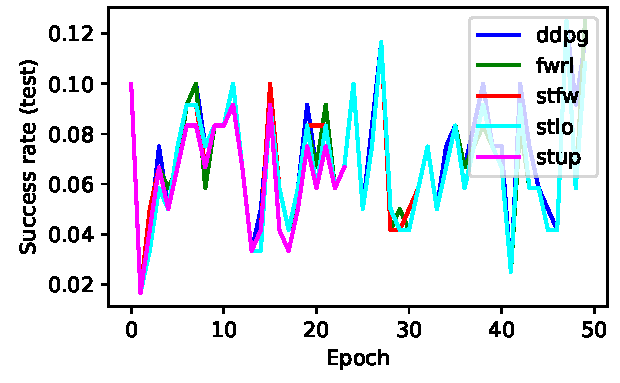
\includegraphics[width=\frac\columnwidth]{media/res/f84daa7-FetchPush-v1-stfw-none/test/success_rate.pdf}%
  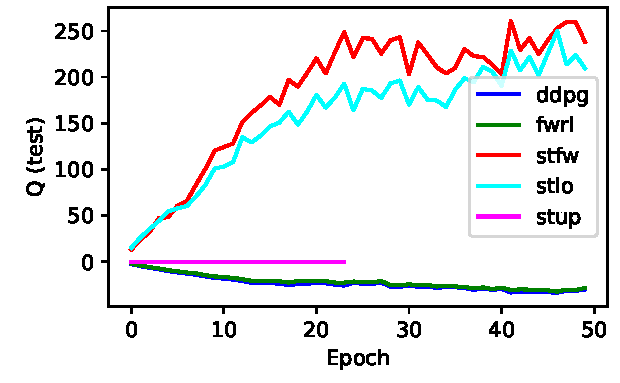
\includegraphics[width=\frac\columnwidth]{media/res/f84daa7-FetchPush-v1-stfw-none/test/mean_Q.pdf}%
  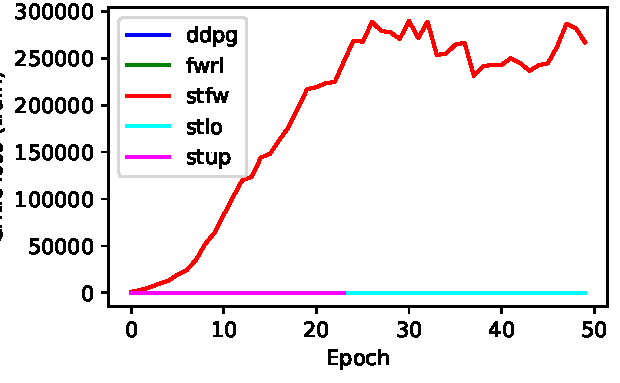
\includegraphics[width=\frac\columnwidth]{media/res/f84daa7-FetchPush-v1-stfw-none/train/critic_loss.pdf}\\
Loss function breakdown with HER sampling on Fetch Push\\
  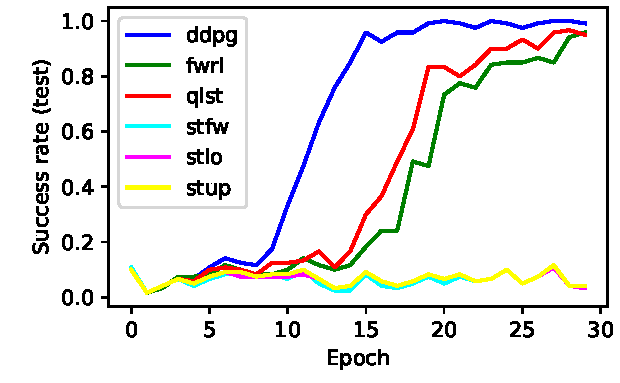
\includegraphics[width=\frac\columnwidth]{media/res/3f1eafe-FetchPush-v1-stfw-future/test/success_rate.pdf}%
  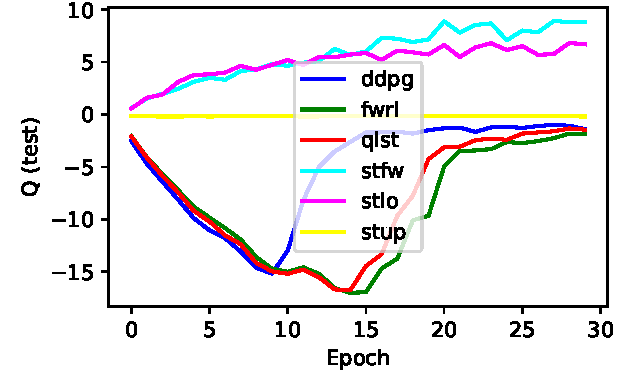
\includegraphics[width=\frac\columnwidth]{media/res/3f1eafe-FetchPush-v1-stfw-future/test/mean_Q.pdf}%
  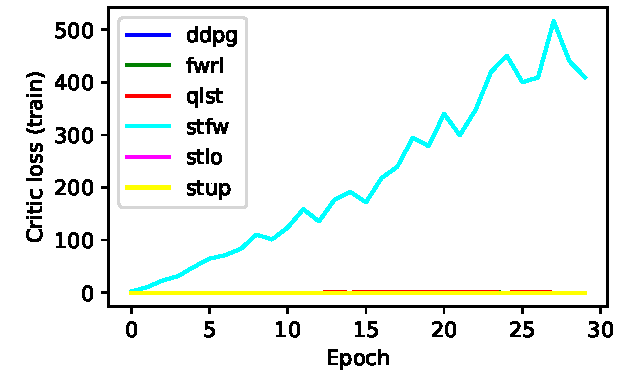
\includegraphics[width=\frac\columnwidth]{media/res/3f1eafe-FetchPush-v1-stfw-future/train/critic_loss.pdf}%
  \caption{
    Fetch Push results. Loss function changes do no seem to make a difference.
    There are four parts to the loss function (1) DDPG Loss $\Loss_{\text{ddpg}}$ ,
    (2) Step loss$\Loss_{\text{step}}$,  
    (3) Lower bound $\Loss_{\text{lower}}$ and
    (4) Upper bound $\Loss_{\text{upper}}$ .
    ddpg = $\Loss_{\text{ddpg}}$,
    dqst = $\Loss_{\text{ddpg}}$ + $\Loss_{\text{step}}$,
    fwrl = $\Loss_{\text{ddpg}}$ + $\Loss_{\text{lower}}$ +
    $\Loss_{\text{upper}}$,
    qlst = $\Loss_{\text{ddpg}}$ + $\Loss_{\text{step}}$ + $\Loss_{\text{lower}}$ + $\Loss_{\text{upper}}$.
    stfw = $\Loss_{\text{step}}$ + $\Loss_{\text{lower}}$ + $\Loss_{\text{upper}}$,
    stlo = $\Loss_{\text{step}}$ + $\Loss_{\text{lower}}$,
    stup = $\Loss_{\text{step}}$ + $\Loss_{\text{upper}}$.
    Success rate is the fraction of times the agent reaches the goal. Q(test) is
    the estimated cumulative reward by the network. Critic loss is the total
    loss plotted during training.
    Because stfw, stlo, stup fail to succeed, we infer that the $\Loss_{\text{ddpg}}$ DDPG loss is
    critical for making the algorithm work. Since the qlst works better than
    fwrl, we infer that $\Loss_{\text{step}}$ Step loss is also important.
    only.
    Since there is slight improvement in dqst over ddpg, this means
    $\Loss_{\text{step}}$ really helps. dqst did not run fully but it shows
    promise (I need to fix a bug).
    But why does the loss for stfw keep rising? Does it mean that the SGD is not
    able to optimize the loss gradients in the right direction?
  }%
  \label{fig:fwrl-stepfwrl-noop-FetchPush}%
\end{figure}%
% 


\subsection{Unanswered questions and things to try}

\subsubsection{FWRL specific sampling}
Right now the shuffle step in the algorithm is totally random and probably
introduces more noise in the algorithm than it helps. A modification of HER
sampling would sampling three time steps from the trajectory (single episode)
$t_1 > t_2 > t_3$ and use $t_2$ as the intermediate state for
$\Loss_{\text{upper}}$ and $\Loss_{\text{lower}}$.


\subsubsection{Why is any loss term with upper/lower worse?}
This is probably answered by  the above section but what are the other
explanations. The total ``Critic loss'' is increasing for stfw
($=\Loss_{\text{step}}$ + $\Loss_{\text{lower}}$ + $\Loss_{\text{upper}}$),
which seems to say that with $\Loss_{\text{ddpg}}$, it is hard to optimize the functions.


\subsection{Is it still a contribution if the upper and lower bounds do not
  improve the results?}
Can we claim that this alternative formulation is new and more principled than HER?

\section{Old Experiments}
%
\subsection{Notation}

\begin{tabular}{ll}   
  \toprule
  Symbol & Meaning\\
  \midrule
  $\state \in \State$ & State $\state$ in state space $\State$ \\
  $\act \in \Action$ & Action $\act$ in Action space $\Action$ \\
  $\rew \in \R$ & Observed reward \\
  $\goal \in \Goal$ & Goal $\goal$ in goal space $\Goal$ \\
  $f_\goal(\state_t): \State \rightarrow \Goal$ & Function to compute achieved goal \\
  $\Rew(\state, \act) : \State \times \Action \rightarrow \R $ & Reward function \\
  $\Rew(\state, \goal, \act) : \State \times \Goal \times \Action \rightarrow \R $ & Goal-conditioned Reward function \\
  $\TransFull$ & Transition function \\
  $\discount$ & Discount factor \\
  MDP=$(\State, \Action, \Trans, \Rew, \discount)$& Markov Decision Process \\
  $\policy(\state): \State \rightarrow \Action $ & Policy function \\
  $\policy(\state, \goal): \State \times \Goal \rightarrow \Action $ & Goal conditioned Policy function \\
  $\Q_\policy(\state, \act; \param_\Q) = \E_\policy[ \sum_{k=t}^\infty \discount^{k-t} \Rew(\state_k, \act_k) | \state_t = \state, \act_t = \act ] $ & $Q$-function \\
  $\Q^*(\state, \act; \param_\Q) = \arg \max_\policy \Q_\policy(\state, \act; \param_\Q)$ & Optimal $Q$-function \\
  $\fwargs{\state}{\act}{\goal^*}{\policy}{} = \E_\policy[ \sum_{k=t}^\infty \discount^{k-t}\Rew(\state_k, \goal^*, \act_k) | \state_t = \state, \act_t = \act]$ & Goal conditioned Q-function \\
  \bottomrule
\end{tabular}
\begin{figure}%
  \def\frac{0.24}
  On Fetch Reach\\
  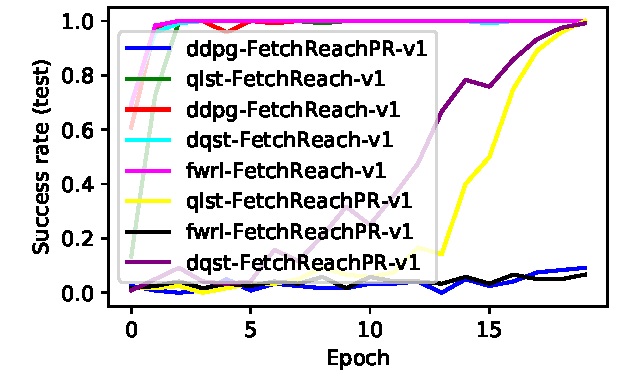
\includegraphics[width=\frac\columnwidth]{media/res/245b3c4-ce781a70-FetchReachPR-v1-fwrl-future-her_fwrl_path_reward/test/success_rate.pdf}%
  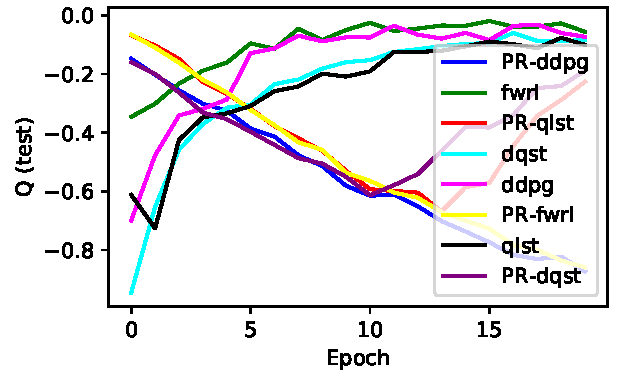
\includegraphics[width=\frac\columnwidth]{media/res/245b3c4-ce781a70-FetchReachPR-v1-fwrl-future-her_fwrl_path_reward/test/mean_Q.pdf}%
  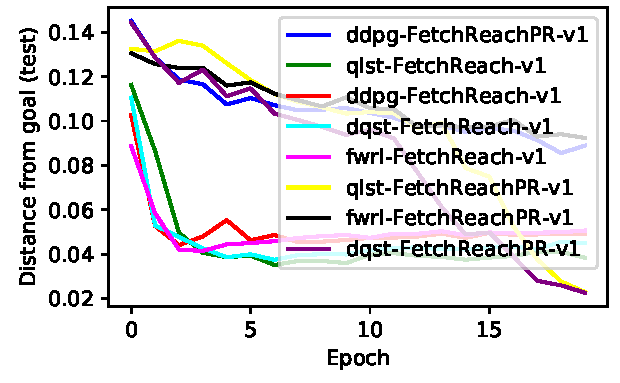
\includegraphics[width=\frac\columnwidth]{media/res/245b3c4-ce781a70-FetchReachPR-v1-fwrl-future-her_fwrl_path_reward/test/ag_g_dist.pdf}%
  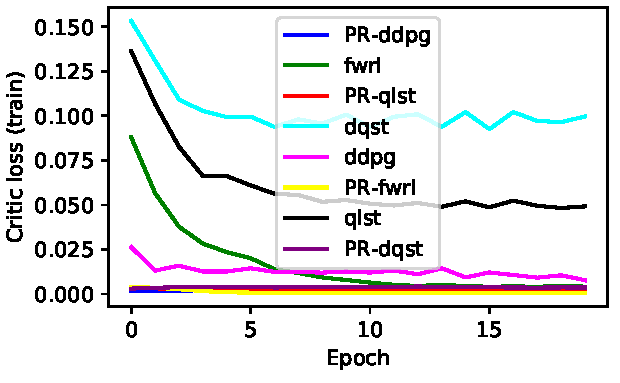
\includegraphics[width=\frac\columnwidth]{media/res/245b3c4-ce781a70-FetchReachPR-v1-fwrl-future-her_fwrl_path_reward/train/critic_loss.pdf}\\
  On Fetch Push\\
  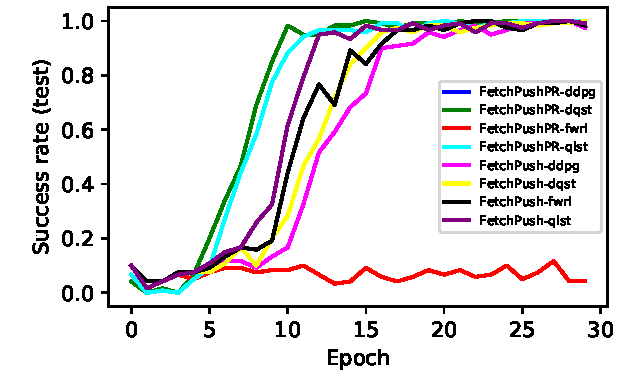
\includegraphics[width=\frac\columnwidth]{./media/res/be0910c-her_fwrl_path_reward-FetchPushPR-v1-fwrl/test/success_rate.pdf}%
  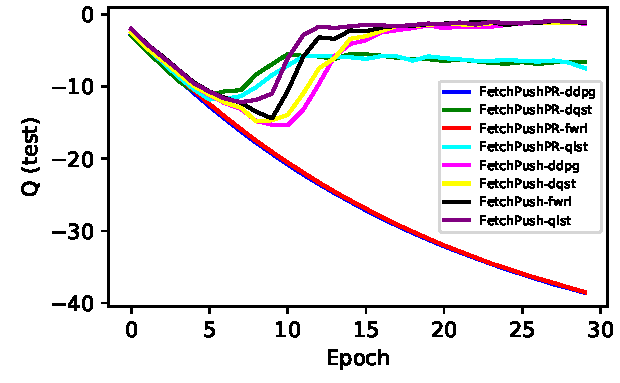
\includegraphics[width=\frac\columnwidth]{./media/res/be0910c-her_fwrl_path_reward-FetchPushPR-v1-fwrl/test/mean_Q.pdf}%
  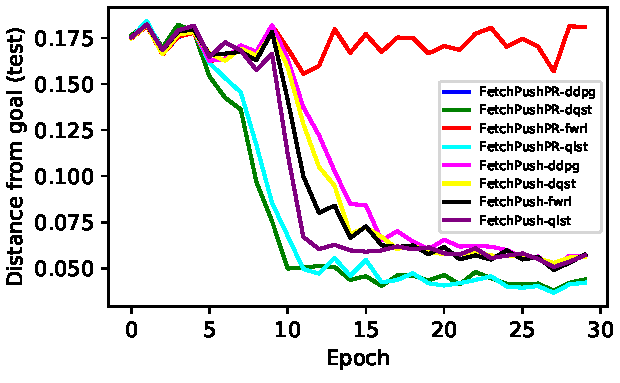
\includegraphics[width=\frac\columnwidth]{./media/res/be0910c-her_fwrl_path_reward-FetchPushPR-v1-fwrl/test/ag_g_dist.pdf}%
  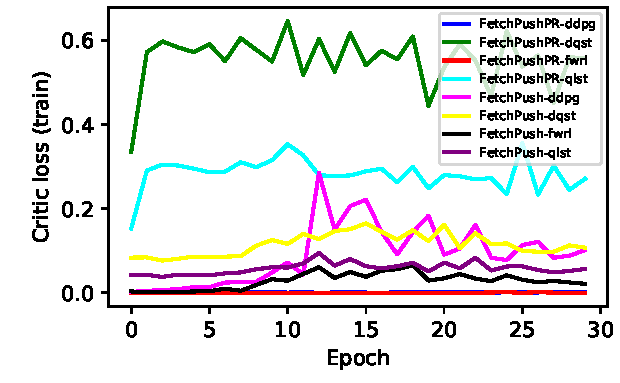
\includegraphics[width=\frac\columnwidth]{./media/res/be0910c-her_fwrl_path_reward-FetchPushPR-v1-fwrl/train/critic_loss.pdf}\\
  On Fetch Slide\\
  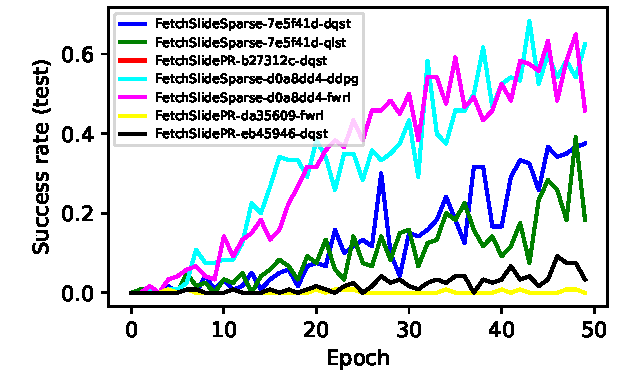
\includegraphics[width=\frac\columnwidth]{./media/res/eb45946-path_reward-FetchSlidePR-v1-dqst/test/success_rate.pdf}%
  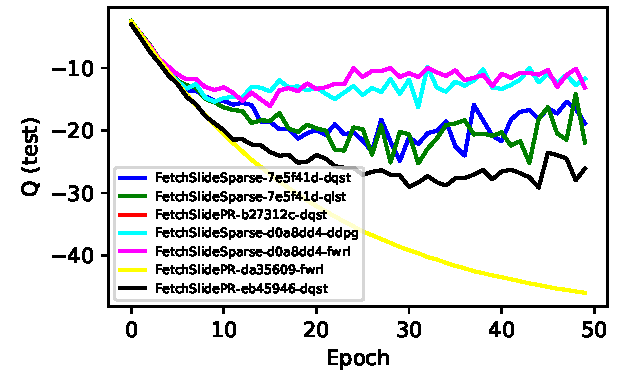
\includegraphics[width=\frac\columnwidth]{./media/res/eb45946-path_reward-FetchSlidePR-v1-dqst/test/mean_Q.pdf}%
  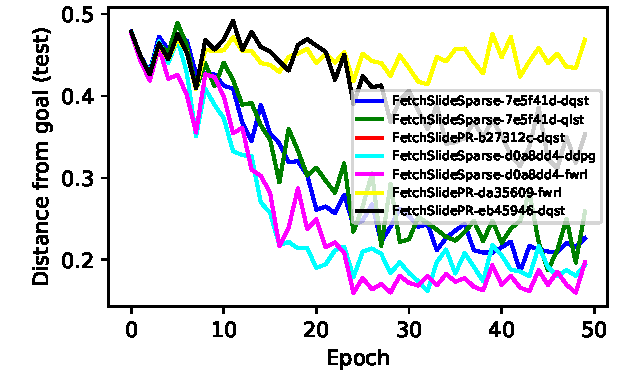
\includegraphics[width=\frac\columnwidth]{./media/res/eb45946-path_reward-FetchSlidePR-v1-dqst/test/ag_g_dist.pdf}%
  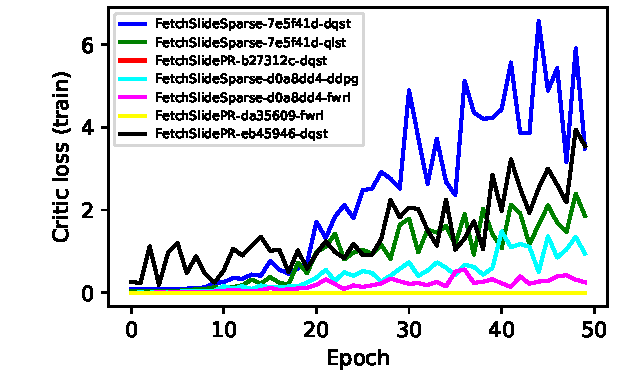
\includegraphics[width=\frac\columnwidth]{./media/res/eb45946-path_reward-FetchSlidePR-v1-dqst/train/critic_loss.pdf}\\
  On Fetch Pick And Place\\
  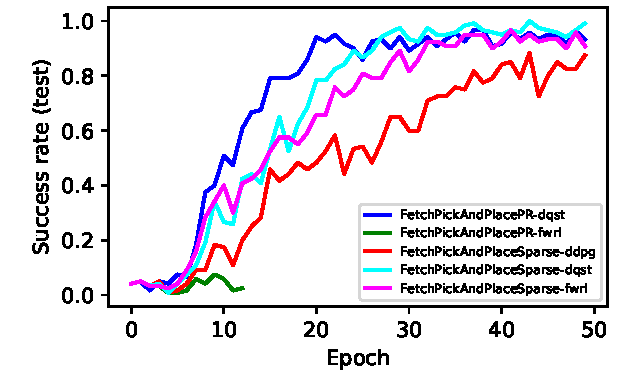
\includegraphics[width=\frac\columnwidth]{./media/res/d5cefef-path_reward-FetchPickAndPlacePR-v1-dqst/test/success_rate.pdf}%
  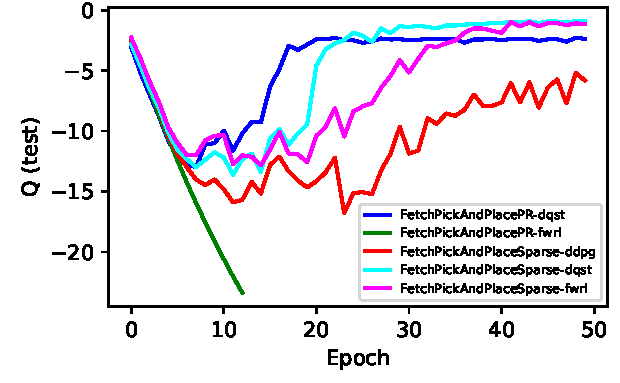
\includegraphics[width=\frac\columnwidth]{./media/res/d5cefef-path_reward-FetchPickAndPlacePR-v1-dqst/test/mean_Q.pdf}%
  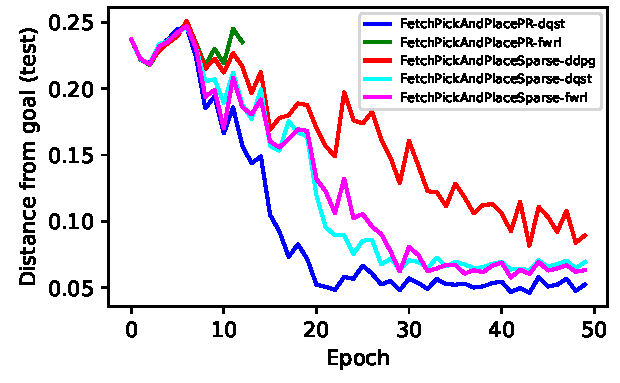
\includegraphics[width=\frac\columnwidth]{./media/res/d5cefef-path_reward-FetchPickAndPlacePR-v1-dqst/test/ag_g_dist.pdf}%
  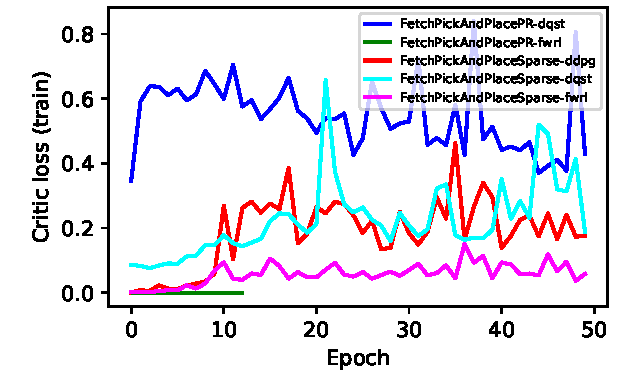
\includegraphics[width=\frac\columnwidth]{./media/res/d5cefef-path_reward-FetchPickAndPlacePR-v1-dqst/train/critic_loss.pdf}\\
  On Hand Reach \\
  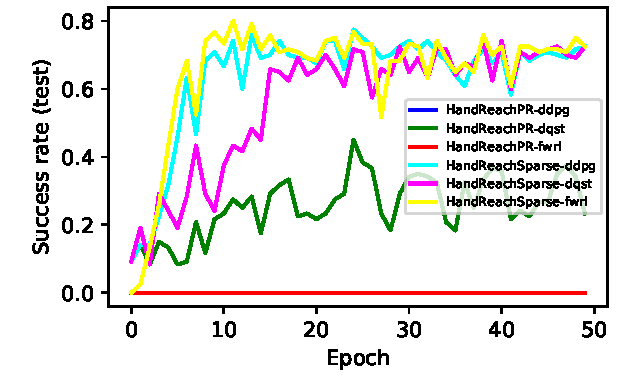
\includegraphics[width=\frac\columnwidth]{./media/res/d5cefef-path_reward-HandReachPR-v0-dqst/test/success_rate.pdf}%
  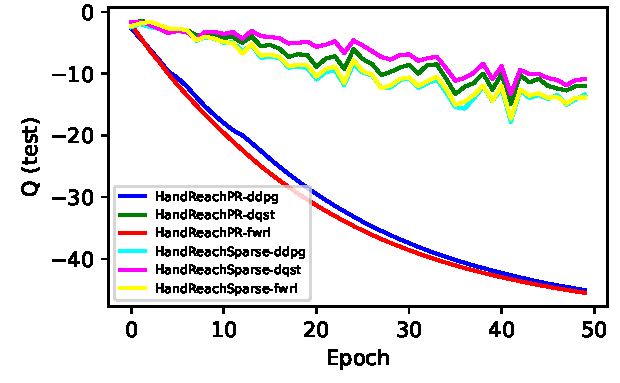
\includegraphics[width=\frac\columnwidth]{./media/res/d5cefef-path_reward-HandReachPR-v0-dqst/test/mean_Q.pdf}%
  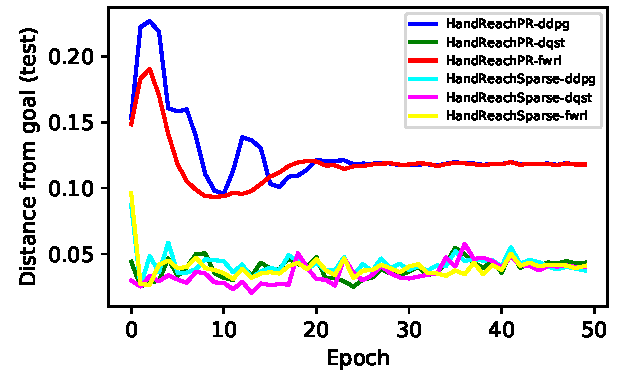
\includegraphics[width=\frac\columnwidth]{./media/res/d5cefef-path_reward-HandReachPR-v0-dqst/test/ag_g_dist.pdf}%
  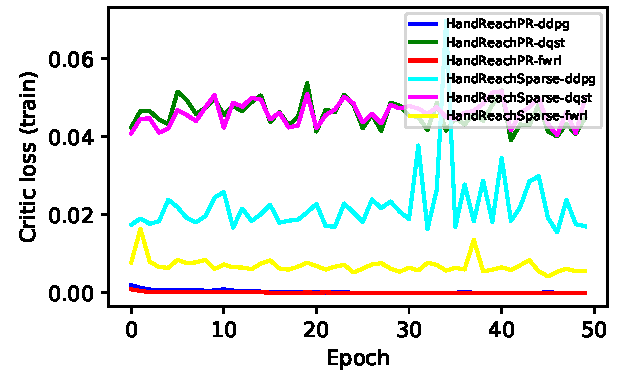
\includegraphics[width=\frac\columnwidth]{./media/res/d5cefef-path_reward-HandReachPR-v0-dqst/train/critic_loss.pdf}\\
  \label{fig:path-reward-1}%
  \caption{Effect of path reward on convergence in case of different loss
    functions on FetchReach. With path reward on PR-dqst
    ($\LossDDPG$ + $\LossStep$)
    and PR-qlst
    ($\LossDDPG$ + $\LossStep$ + $\LossLo$ + $\LossUp$), are able achieve high
    success rate and even that takes longer than usual. Out of the two PR-dqst
    does better. The terms with PR use path-rewards and hence less computation
    by avoid recomputation of reward function. It is interesting that PR-dqst
    and PR-qlst reach closer in terms of distance from goal probably because of
    absence of threshold.}%
\end{figure}%
% 

\begin{figure}
  \def\frac{0.32}
    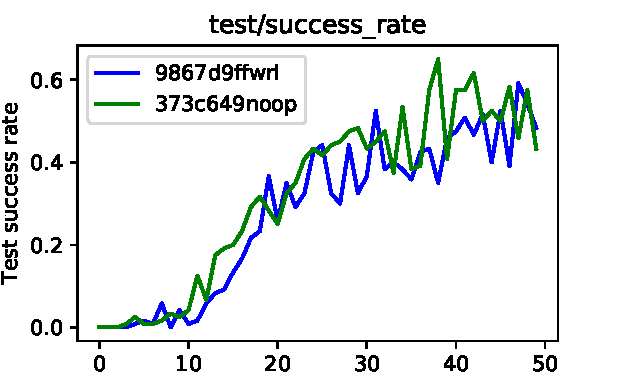
\includegraphics[width=\frac\columnwidth]{media/res/373c649_FetchSlide-v1-noop/test/success_rate.pdf}%
    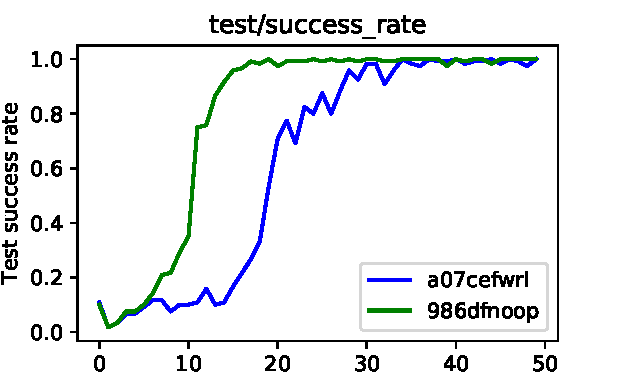
\includegraphics[width=\frac\columnwidth]{media/res/a077c9e_FetchPush-v1-fwrl/test/success_rate.pdf}%
    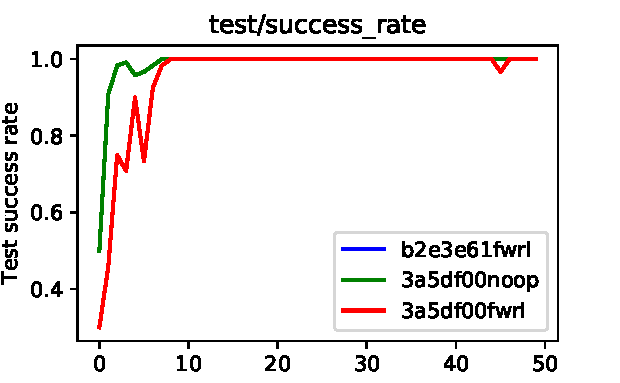
\includegraphics[width=\frac\columnwidth]{media/res/3a5df00_FetchReach-v1-fwrl/test/success_rate.pdf}\\
    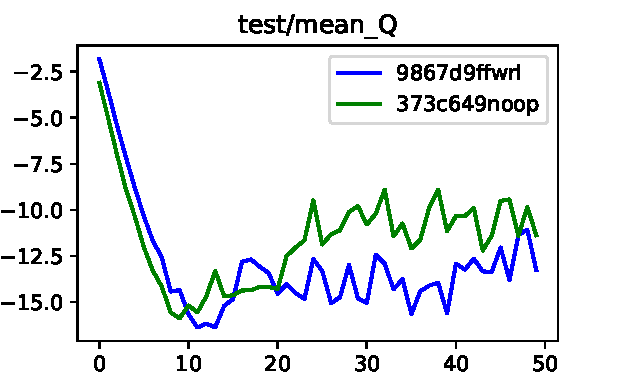
\includegraphics[width=\frac\columnwidth]{media/res/373c649_FetchSlide-v1-noop/test/mean_Q.pdf}%
    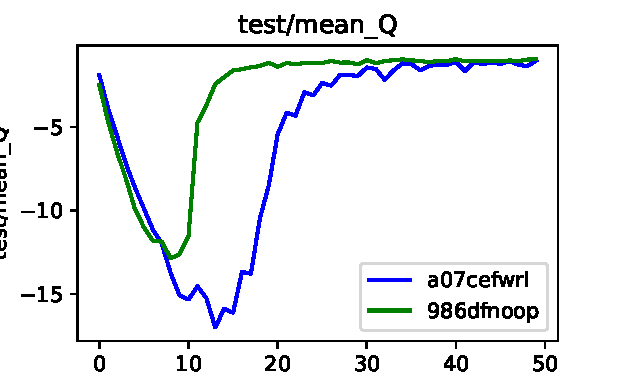
\includegraphics[width=\frac\columnwidth]{media/res/a077c9e_FetchPush-v1-fwrl/test/mean_Q.pdf}%
    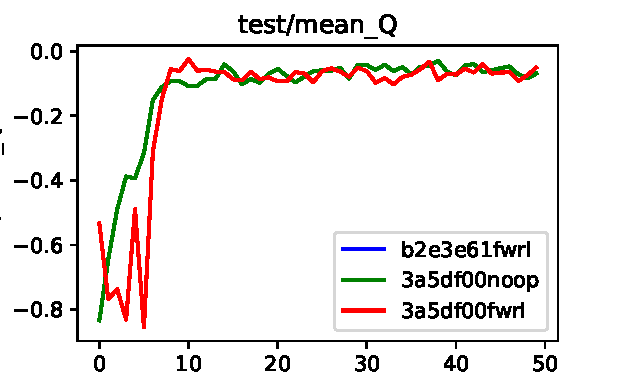
\includegraphics[width=\frac\columnwidth]{media/res/3a5df00_FetchReach-v1-fwrl/test/mean_Q.pdf}
    \caption{fwrl = Floyd Warshall ($=\Loss_{\text{ddpg}} +
      \Loss_{\text{upper}}$) with HER sampling;
      noop = DDPG ($=\Loss_{\text{ddpg}}$)with HER sampling.
  Test success rate and Mean Q on (1) Fetch-Slide, (2) Fetch-Push and (3)
  Fetch-Reach task. fwrl does consistently worse than HER.}
    \label{fig:fetch-slide-success}
\end{figure}


%
\begin{figure}%
  \def\frac{0.24}
  With HER sampling:\\
  \includegraphics[width=\frac\columnwidth]{media/res/3a90344-FetchReach-v1-stepfwrl-future/test/success_rate.pdf}%
  \includegraphics[width=\frac\columnwidth]{media/res/3a90344-FetchReach-v1-stepfwrl-future/test/mean_Q.pdf}%
  \includegraphics[width=\frac\columnwidth]{media/res/3a90344-FetchReach-v1-stepfwrl-future/train/critic_loss.pdf}%
  \includegraphics[width=\frac\columnwidth]{media/res/3a90344-FetchReach-v1-stepfwrl-future/train/critic_addnl_loss.pdf}\\
  Without HER sampling:\\
  \includegraphics[width=\frac\columnwidth]{media/res/d047a03-FetchReach-v1-stepfwrl-none/test/success_rate.pdf}%
  \includegraphics[width=\frac\columnwidth]{media/res/d047a03-FetchReach-v1-stepfwrl-none/test/mean_Q.pdf}%
  \includegraphics[width=\frac\columnwidth]{media/res/d047a03-FetchReach-v1-stepfwrl-none/train/critic_loss.pdf}%
  \includegraphics[width=\frac\columnwidth]{media/res/d047a03-FetchReach-v1-stepfwrl-none/train/critic_addnl_loss.pdf}\\
Using both upper and lower bound in FWRL\\
  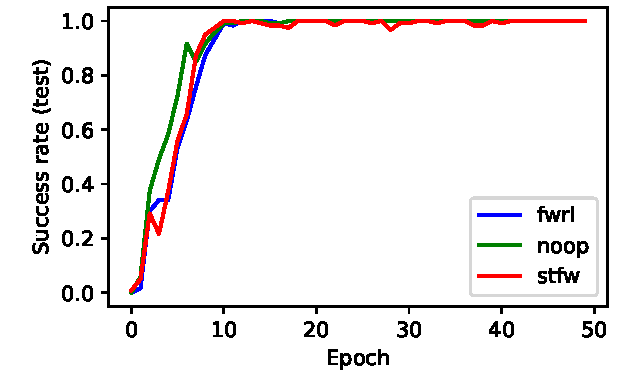
\includegraphics[width=\frac\columnwidth]{media/res/f0d4cfa-FetchReach-v1-stfw-none/test/success_rate.pdf}%
  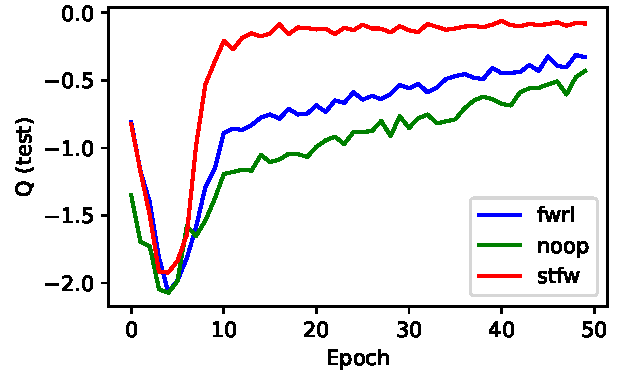
\includegraphics[width=\frac\columnwidth]{media/res/f0d4cfa-FetchReach-v1-stfw-none/test/mean_Q.pdf}%
  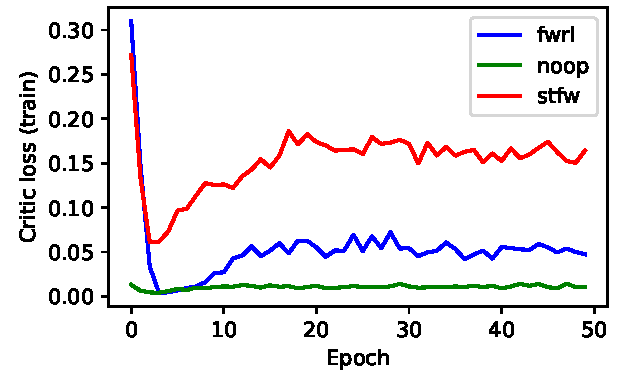
\includegraphics[width=\frac\columnwidth]{media/res/f0d4cfa-FetchReach-v1-stfw-none/train/critic_loss.pdf}%
  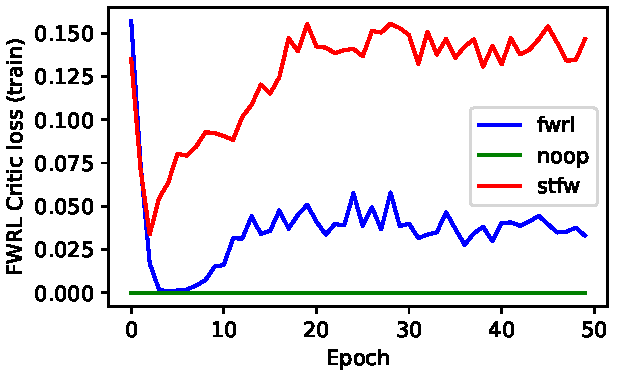
\includegraphics[width=\frac\columnwidth]{media/res/f0d4cfa-FetchReach-v1-stfw-none/train/critic_addnl_loss.pdf}\\
  \caption{
    stepfwrl = DDPG loss $\Loss_{\text{ddpg}}$ + Step loss $\Loss_{\text{step}}$
    + FWRL constraints $\Loss_{\text{upper}} + \Loss_{\text{lower}}$, noop =
    DDPG loss $\Loss_{\text{ddpg}}$  + HER
    sampling, fwrl = DDPG Loss $\Loss_{\text{ddpg}}$ + FWRL constraints $\Loss_{\text{upper}} + \Loss_{\text{lower}}$.
    All experiments on Fetch-Reach task.
  }%
  \label{fig:fwrl-stepfwrl-noop-FetchReach}%
\end{figure}%
% 

%
\begin{figure}%
  \def\frac{0.24}
  With HER sampling\\
  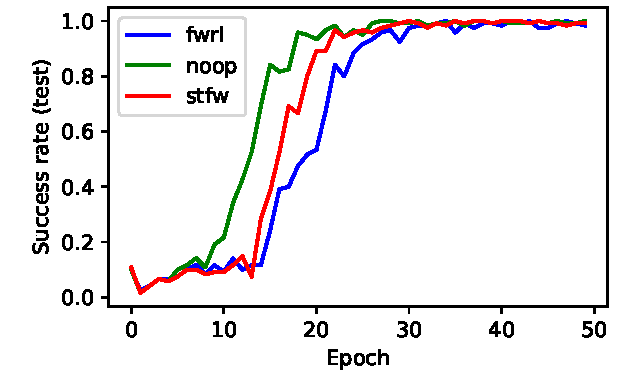
\includegraphics[width=\frac\columnwidth]{media/res/ea0e35b-FetchPush-v1-stfw-future/test/success_rate.pdf}%
  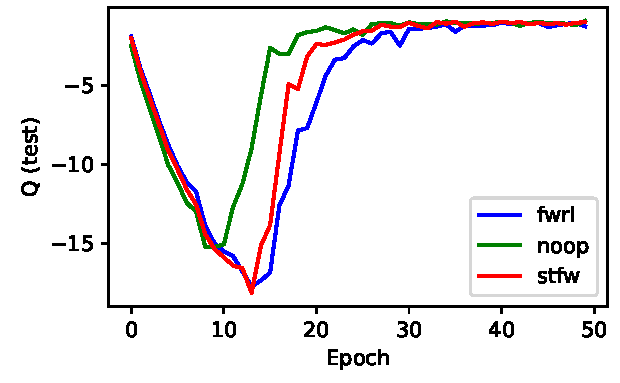
\includegraphics[width=\frac\columnwidth]{media/res/ea0e35b-FetchPush-v1-stfw-future/test/mean_Q.pdf}%
  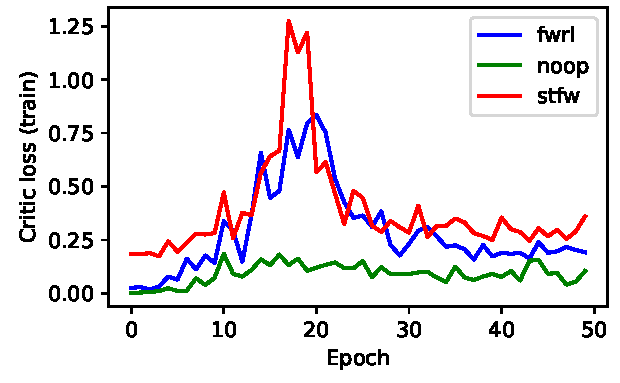
\includegraphics[width=\frac\columnwidth]{media/res/ea0e35b-FetchPush-v1-stfw-future/train/critic_loss.pdf}%
  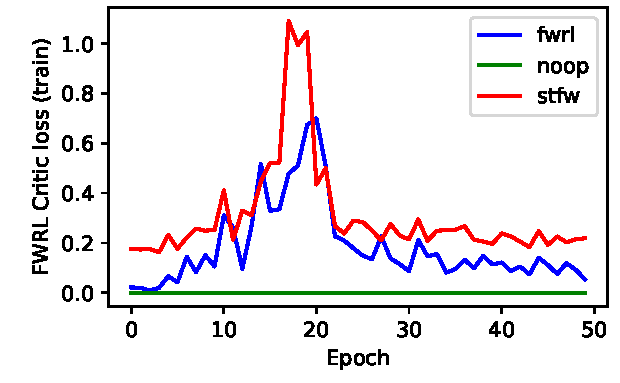
\includegraphics[width=\frac\columnwidth]{media/res/ea0e35b-FetchPush-v1-stfw-future/train/critic_addnl_loss.pdf}\\
  Without HER sampling\\
  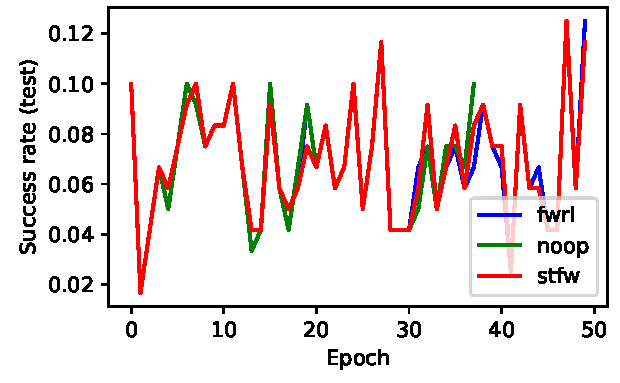
\includegraphics[width=\frac\columnwidth]{media/res/ea0e35b-FetchPush-v1-stfw-none/test/success_rate.pdf}%
  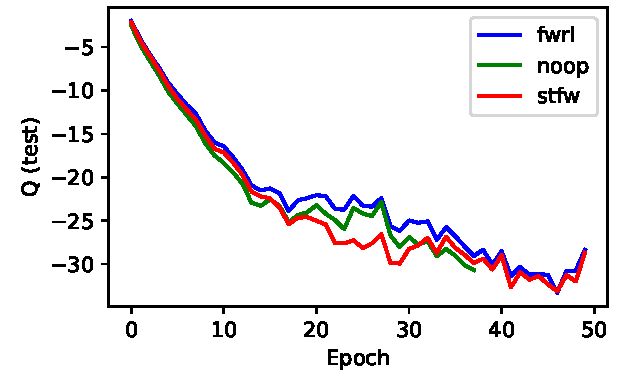
\includegraphics[width=\frac\columnwidth]{media/res/ea0e35b-FetchPush-v1-stfw-none/test/mean_Q.pdf}%
  \includegraphics[width=\frac\columnwidth]{media/res/ea0e35b-FetchPush-v1-stfw-none/train/critic_loss.pdf}%
  \includegraphics[width=\frac\columnwidth]{media/res/ea0e35b-FetchPush-v1-stfw-none/train/critic_addnl_loss.pdf}%
  \caption{stepfwrl = DDPG loss $\Loss_{\text{ddpg}}$ + Step loss $\Loss_{\text{step}}$
    + FWRL constraints $\Loss_{\text{upper}} + \Loss_{\text{lower}}$, noop =
    DDPG loss $\Loss_{\text{ddpg}}$  + HER
    sampling, fwrl = DDPG Loss $\Loss_{\text{ddpg}}$ + FWRL constraints $\Loss_{\text{upper}} + \Loss_{\text{lower}}$.
    All experiments on Fetch-Push}
  \label{fig:loss-func-fetch-push}
\end{figure}
%

%
\begin{figure}
  \def\frac{0.32}
Loss function breakdown without HER sampling on Fetch Push\\
  \includegraphics[width=\frac\columnwidth]{media/res/f84daa7-FetchPush-v1-stfw-none/test/success_rate.pdf}%
  \includegraphics[width=\frac\columnwidth]{media/res/f84daa7-FetchPush-v1-stfw-none/test/mean_Q.pdf}%
  \includegraphics[width=\frac\columnwidth]{media/res/f84daa7-FetchPush-v1-stfw-none/train/critic_loss.pdf}\\
Loss function breakdown with HER sampling on Fetch Push\\
  \includegraphics[width=\frac\columnwidth]{media/res/3f1eafe-FetchPush-v1-stfw-future/test/success_rate.pdf}%
  \includegraphics[width=\frac\columnwidth]{media/res/3f1eafe-FetchPush-v1-stfw-future/test/mean_Q.pdf}%
  \includegraphics[width=\frac\columnwidth]{media/res/3f1eafe-FetchPush-v1-stfw-future/train/critic_loss.pdf}%
  \caption{
    Fetch Push results. Loss function changes do no seem to make a difference.
    There are four parts to the loss function (1) DDPG Loss $\Loss_{\text{ddpg}}$ ,
    (2) Step loss$\Loss_{\text{step}}$,  
    (3) Lower bound $\Loss_{\text{lower}}$ and
    (4) Upper bound $\Loss_{\text{upper}}$ .
    ddpg = $\Loss_{\text{ddpg}}$,
    dqst = $\Loss_{\text{ddpg}}$ + $\Loss_{\text{step}}$,
    fwrl = $\Loss_{\text{ddpg}}$ + $\Loss_{\text{lower}}$ +
    $\Loss_{\text{upper}}$,
    qlst = $\Loss_{\text{ddpg}}$ + $\Loss_{\text{step}}$ + $\Loss_{\text{lower}}$ + $\Loss_{\text{upper}}$.
    stfw = $\Loss_{\text{step}}$ + $\Loss_{\text{lower}}$ + $\Loss_{\text{upper}}$,
    stlo = $\Loss_{\text{step}}$ + $\Loss_{\text{lower}}$,
    stup = $\Loss_{\text{step}}$ + $\Loss_{\text{upper}}$.
    Success rate is the fraction of times the agent reaches the goal. Q(test) is
    the estimated cumulative reward by the network. Critic loss is the total
    loss plotted during training.
    Because stfw, stlo, stup fail to succeed, we infer that the $\Loss_{\text{ddpg}}$ DDPG loss is
    critical for making the algorithm work. Since the qlst works better than
    fwrl, we infer that $\Loss_{\text{step}}$ Step loss is also important.
    only.
    Since there is slight improvement in dqst over ddpg, this means
    $\Loss_{\text{step}}$ really helps. dqst did not run fully but it shows
    promise (I need to fix a bug).
    But why does the loss for stfw keep rising? Does it mean that the SGD is not
    able to optimize the loss gradients in the right direction?
  }%
  \label{fig:fwrl-stepfwrl-noop-FetchPush}%
\end{figure}%
% 

%
\begin{figure}
  \def\frac{0.32}
  On Fetch Push\\
  \includegraphics[width=\frac\columnwidth]{media/res/38f4625-FetchPush-v1-fwrl-future/test/success_rate.pdf}%
  \includegraphics[width=\frac\columnwidth]{media/res/38f4625-FetchPush-v1-fwrl-future/test/mean_Q.pdf}%
  \includegraphics[width=\frac\columnwidth]{media/res/38f4625-FetchPush-v1-fwrl-future/train/critic_loss.pdf}\\
  On Fetch Reach\\
  \includegraphics[width=\frac\columnwidth]{media/res/38f4625-FetchReach-v1-fwrl-future/test/success_rate.pdf}%
  \includegraphics[width=\frac\columnwidth]{media/res/38f4625-FetchReach-v1-fwrl-future/test/mean_Q.pdf}%
  \includegraphics[width=\frac\columnwidth]{media/res/38f4625-FetchReach-v1-fwrl-future/train/critic_loss.pdf}\\
  On Fetch Slide\\
  \includegraphics[width=\frac\columnwidth]{media/res/38f4625-FetchSlide-v1-fwrl-future/test/success_rate.pdf}%
  \includegraphics[width=\frac\columnwidth]{media/res/38f4625-FetchSlide-v1-fwrl-future/test/mean_Q.pdf}%
  \includegraphics[width=\frac\columnwidth]{media/res/38f4625-FetchSlide-v1-fwrl-future/train/critic_loss.pdf}%
  On Fetch Pick and Place\\
  \includegraphics[width=\frac\columnwidth]{media/res/38f4625-FetchPickAndPlace-v1-fwrl-future/test/success_rate.pdf}%
  \includegraphics[width=\frac\columnwidth]{media/res/38f4625-FetchPickAndPlace-v1-fwrl-future/test/mean_Q.pdf}%
  \includegraphics[width=\frac\columnwidth]{media/res/38f4625-FetchPickAndPlace-v1-fwrl-future/train/critic_loss.pdf}%
  On HandReach\\
  \includegraphics[width=\frac\columnwidth]{media/res/38f4625-92450888-HandReach-v0-fwrl-future/test/success_rate.pdf}%
  \includegraphics[width=\frac\columnwidth]{media/res/38f4625-92450888-HandReach-v0-fwrl-future/test/mean_Q.pdf}%
  \includegraphics[width=\frac\columnwidth]{media/res/38f4625-92450888-HandReach-v0-fwrl-future/train/critic_loss.pdf}%
  \caption{
    Fetch results. Loss function changes do no seem to make a difference.
    There are four parts to the loss function (1) DDPG Loss $\LossDDPG$ ,
    (2) Step loss$\LossStep$,  
    (3) Lower bound $\LossLo$ and
    (4) Upper bound $\LossUp$ .
    ddpg = $\LossDDPG$,
    dqst = $\LossDDPG$ + $\LossStep$,
    fwrl = $\LossDDPG$ + $\LossLo$ +
    $\LossUp$,
    qlst = $\LossDDPG$ + $\LossStep$ + $\LossLo$ + $\LossUp$,
    dqte = $\LossDDPG$ + $\LossTrieq$,
    qste = $\LossDDPG$ + $\LossStep$ + $\LossTrieq$.
    Success rate is the fraction of times the agent reaches the goal. Q(test) is
    the estimated cumulative reward by the network. Critic loss is the total
    loss plotted during training.
    Because stfw, stlo, stup fail to succeed, we infer that the $\LossDDPG$ DDPG loss is
    critical for making the algorithm work. Since the qlst works better than
    fwrl, we infer that $\LossStep$ Step loss is also important.
    only.
    Since there is slight improvement in dqst over ddpg, this means
    $\LossStep$ really helps. dqst did not run fully but it shows
    promise (I need to fix a bug).
    But why does the loss for stfw keep rising? Does it mean that the SGD is not
    able to optimize the loss gradients in the right direction?
  }%
  \label{fig:fwrl-stepfwrl-noop-FetchPush}%
\end{figure}%
% 

%
\begin{figure}%
  \def\frac{0.25}
  \includegraphics[width=\frac\columnwidth]{media/res/3d07a6e-FetchReachPR-v1-fwrl-future/test/success_rate.pdf}%
  \includegraphics[width=\frac\columnwidth]{media/res/3d07a6e-FetchReachPR-v1-fwrl-future/test/mean_Q.pdf}%
  \includegraphics[width=\frac\columnwidth]{media/res/3d07a6e-FetchReachPR-v1-fwrl-future/test/ag_g_dist.pdf}%
  \includegraphics[width=\frac\columnwidth]{media/res/3d07a6e-FetchReachPR-v1-fwrl-future/train/critic_loss.pdf}%
  \label{fig:path-rewards}%
  \caption{Experiment to see the effect of only path rewards on loss terms. We
    did not include a step term which becomes very important in this case.}%
\end{figure}%
% 

%
\begin{figure}%
  \def\frac{0.24}
  \includegraphics[width=\frac\columnwidth]{./media/res/04a8fc6-814a3d24-FetchSlide-v1-fwrl-future/test/success_rate.pdf}%
  \includegraphics[width=\frac\columnwidth]{./media/res/04a8fc6-814a3d24-FetchSlide-v1-fwrl-future/test/mean_Q.pdf}%
  \includegraphics[width=\frac\columnwidth]{./media/res/04a8fc6-814a3d24-FetchSlide-v1-fwrl-future/test/ag_g_dist.pdf}%
  \includegraphics[width=\frac\columnwidth]{./media/res/04a8fc6-814a3d24-FetchSlide-v1-fwrl-future/train/critic_loss.pdf}%
  \label{fig:loss-term-weights}%
  \caption{Effect of weighted combination of loss terms on FetchSlide. The three
  loss terms being weighed in order are $[\LossDDPG, \LossLo, \LossUp]$}%
\end{figure}%
% 
We compared weighted combination of loss terms

%
\begin{figure}%
  \def\frac{0.24}
  \includegraphics[width=\frac\columnwidth]{media/res/d249d2d-c9bfa98b-FetchPush-v1-fwrl-future/test/success_rate.pdf}%
  \includegraphics[width=\frac\columnwidth]{media/res/d249d2d-c9bfa98b-FetchPush-v1-fwrl-future/test/mean_Q.pdf}%
  \includegraphics[width=\frac\columnwidth]{media/res/d249d2d-c9bfa98b-FetchPush-v1-fwrl-future/test/ag_g_dist.pdf}%
  \includegraphics[width=\frac\columnwidth]{media/res/d249d2d-c9bfa98b-FetchPush-v1-fwrl-future/train/critic_loss.pdf}%
  \label{fig:middle-vs-uniform}%
  \caption{Effect of choosing the intermediate sample in the \emph{middle} of the
    trajectory vs \emph{uniform}ly random in the trajectory on FetchPush}%
\end{figure}%
% 

%
\begin{figure}%
  \includegraphics[width=\columnwidth]{./media/res/eb45946-path_reward-FetchSlidePR-v1-dqst/test/success_rate.pdf}%
  \label{fig:}%
  \caption{Effect of path rewards on FetchSlide}%
\end{figure}%
% 

%\subsection{Unanswered questions and things to try}
%
%\subsubsection{FWRL specific sampling}
%Right now the shuffle step in the algorithm is totally random and probably
%introduces more noise in the algorithm than it helps. A modification of HER
%sampling would sampling three time steps from the trajectory (single episode)
%$t_1 > t_2 > t_3$ and use $t_2$ as the intermediate state for
%$\LossUp$ and $\LossLo$.
%
%
%\subsubsection{Why is any loss term with upper/lower worse?}
%This is probably answered by  the above section but what are the other
%explanations. The total ``Critic loss'' is increasing for stfw
%($=\LossStep$ + $\LossLo$ + $\LossUp$),
%which seems to say that with $\LossDDPG$, it is hard to optimize the functions.
%
%
%\subsection{Is it still a contribution if the upper and lower bounds do not
%  improve the results?}
%Can we claim that this alternative formulation is new and more principled than HER?